\documentclass{article}
\usepackage{url}
\usepackage{amsmath}
\usepackage{subfiles}
\usepackage{graphicx}
\usepackage{csquotes}

\graphicspath{ {img/} } % path to images

\title{Introduction to Dynamic Programming}
\author{Joshua Saunders}
\date{February 2018}
\begin{document}

\maketitle

\section{Introduction}

After a performance measure for a system has been chosen, we must next choose a
method to minimize it. One technique is \textit{dynamic programming}.

\subsection{Principle of Optimality}

According to Bellman \cite{bellman2015applied},

\begin{displayquote}
An optimal policy has the property that whatever the initial state and initial
decision are, the remaining decisions must constitue an optimal policy with
regard to the state resulting from the first decision.
\end{displayquote}

Figure \ref{fig:optimal_paths} shows a multistage decision process. The first
decision leads from \textit{a} to \textit{b} with a cost of $J_{ab}$.

\begin{figure}[h]
    \begin{center}
        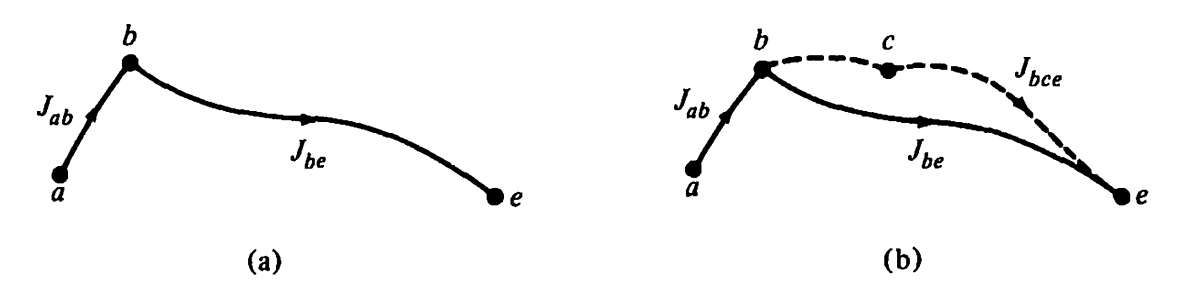
\includegraphics[scale=0.3]{optimality_principle_paths}
        \caption{
          (a) Optimal path from \textit{a} to \textit{e}
          (b) Two possible optimal paths from \textit{b} to \textit{e}
          \cite{kirkdover}
        }
        \label{fig:optimal_paths}
    \end{center}
\end{figure}

\newpage
\bibliography{bib}
\bibliographystyle{ieeetr}

\end{document}
